\section{Auswertung}
\label{sec:Auswertung}

\begin{table}
  \centering
  \caption{Alle aufgenommenen Größen in Abhängigkeit der Zeit in Ablesereihenfolge.}
  \label{tab:messwerte}
  \begin{tblr}{
    colspec={S[table-format=2.2] S[table-format=2.2] S[table-format=2.2] S[table-format=2.2] S[table-format=2.2] 
    S[table-format=2.2]},
    row{1}={guard, mode=math},}
    \toprule
    t\mathbin{/}\unit{\second} & A\mathbin{/}\unit{\watt} & p_{\symup{b}}\mathbin{/}\unit{\bar} & T_1\mathbin{/}°C &
    T_2\mathbin{/}°C & p_{\symup{a}}\mathbin{/}\unit{\bar} \\
    \midrule
    0   &    0    &   3.5   &   20.5  &   20.6  &   3.8   \\       
    1   &    110  &   5     &   21.4  &   20.5  &   3     \\
    2   &    115  &   5     &   22.8  &   19.1  &   3.3   \\
    3   &    120  &   5.5   &   24.2  &   17.8  &   3.4   \\
    4   &    120  &   6     &   25.9  &   16.4  &   3.5   \\
    5   &    120  &   6     &   27.6  &   15.0  &   3.4   \\
    6   &    120  &   6.5   &   28.9  &   14.2  &   3.2   \\
    7   &    120  &   7     &   30.4  &   13.2  &   3     \\
    8   &    120  &   7     &   31.6  &   12.2  &   3     \\
    9   &    125  &   7     &   33.0  &   11.2  &   2.9   \\
    10  &    125  &   7.5   &   34.2  &   10.3  &   2.7   \\
    11  &    125  &   8     &   35.4  &   9.2   &   2.7   \\
    12  &    125  &   8     &   36.5  &   8.4   &   2.6   \\
    13  &    125  &   8     &   37.6  &   7.6   &   2.4   \\
    14  &    125  &   8.5   &   38.6  &   6.7   &   2.4   \\
    15  &    115  &   9     &   39.6  &   5.8   &   2.2   \\
    16  &    115  &   9     &   40.5  &   5.0   &   2.2   \\
    17  &    115  &   9     &   41.4  &   4.3   &   2.1   \\
    18  &    115  &   9.5   &   42.3  &   3.6   &   2     \\
    19  &    115  &   9.5   &   43.1  &   2.9   &   2     \\
    20  &    115  &   10    &   43.9  &   2.2   &   1.9   \\
    21  &    115  &   10    &   44.6  &   1.6   &   1.9   \\ 
    22  &    115  &   10    &   45.4  &   1.0   &   1.8   \\ 
    23  &    110  &   10.5  &   46.0  &   0.4   &   1.8   \\
    24  &    110  &   10.5  &   46.6  &   -0.2  &   1.8   \\ 
    \bottomrule
  \end{tblr}
\end{table} 

\subsection{Temperaturverläufe}
In Abbildung \ref{fig:plot} werden die Temperaturverläufe von $T_1$ und $T_2$ dargestellt.
Hier wurde die Temperatur in Kelvin und die Zeit in Sekunden umgerechnet.
Für beide Verläufe wurde eine Ausgleichsfunktion als quadratisches Polynom gezeichnet.
Diese werden mit der Gleichung
\begin{equation*}
  f=a*t^2+b*t+c+
\end{equation*}
beschrieben.
Dabei sind die Koeffizienten bei $T_1$
\begin{gather}
  a_{\symup{T}1}=\qty{-6.155(0.22)e-6}{\kelvin\per\second\squared}\\
  b_{\symup{T}1}=\qty{0.02742(0.00033)}{\kelvin\per\second}\\
  c_{\symup{T}1}=\qty{293(0.1)}{\kelvin}
  \label{eqn:fkt1}
\end{gather}
und bei $T_2$
\begin{gather}
  a_{\symup{T}2}=\qty{4.122(0.249)e-6}{\kelvin\per\second\squared}\\
  b_{\symup{T}2}=\qty{0.02078(0.00037)}{\kelvin\per\second}\\
  c_{\symup{T}2}=\qty{294.4(0.12)}{\kelvin}
  \label{eqn:fkt2}
\end{gather}
.

\begin{figure}[H]
  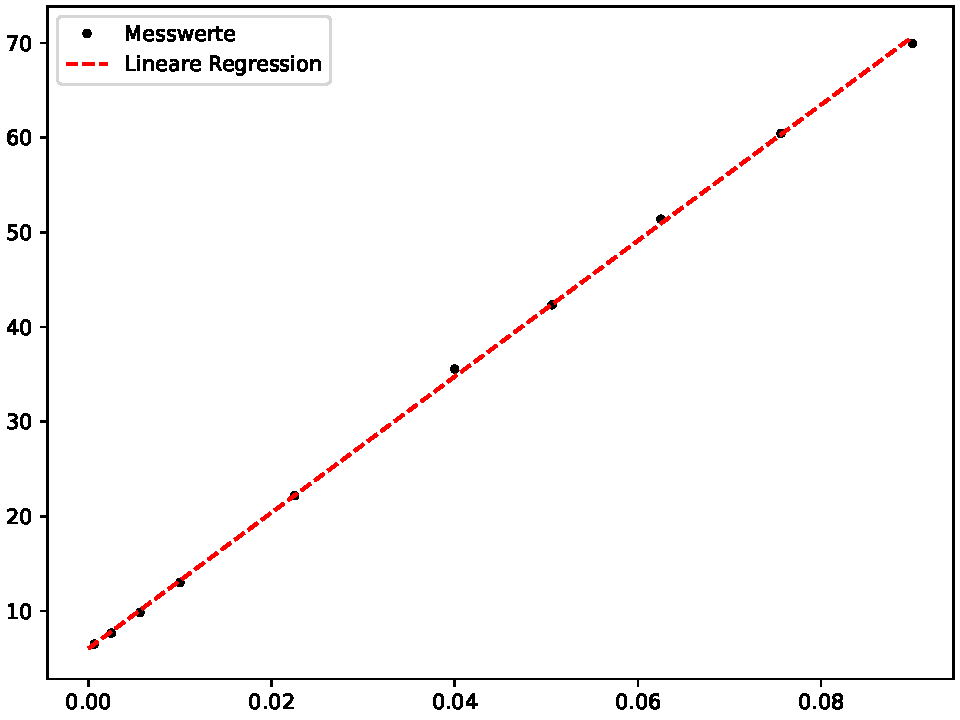
\includegraphics[width=\textwidth]{build/plot.pdf}
  \caption{Dargestellt ist die Temperatur beider Wasserbehälter abhängig von der Zeit. Die Zeit wurde in Sekunden umgerechnet und die Temperatur in Kelvin.}
  \label{fig:plot}
\end{figure}
